\chapter{Thin strip graphs}
\label{chap:thinDef}

The goal of this chapter is to introduce you to the main subject of this thesis. Thin strip graphs is a class of graphs that lay between unit disk graphs
and mixed interval graphs. We can define formally a $c$-strip graph as a unit disk graph such that the centers of the disks belong to $\{(x,y) : -\infty < x < \infty, 0 \leq y \leq c\}$, more intuitively we can see this as a unit disk graph where the centers of the disks lay between two parallel horizontal lines with a distance of $c$ between them. We denote this class by SG($c$). We
have then that SG($0$) = UIG and SG($\infty$) = UDG.

The definition and main work for this class comes from Breu in his thesis \cite{breuAlgorithmicAspectsConstrained1996}. However, Hayashi et al. \cite{hayashiThinStripGraphs2017} expand his work by defining the class of \emph{thin strip graphs}.

\section{Thin strip graphs}

A thin strip graph can be intuitively defined as a $c$-strip graph where $c$ is an arbitrarily little $\varepsilon$. Also, we can see that SG($k$) $\subseteq$ SG($l$) with $k<l$. A more strict definition emerges from this observation:

\begin{defn}
  Thin strip graphs are defined as TSG $= \bigcap_{c > 0}$ SG($c$).
\end{defn}

\begin{remark}
  SG($0$) $\neq$ TSG. We can construct a $K_{1,3}$ such that we have 3 vertices with the coordinates
  $(1,0)$, $(0,0)$, $(1,0)$ and a last one $(0,\varepsilon)$ with $\varepsilon > 0$ and arbitrarily small
  as seen in Figure \ref{fig:thinK13}.
\end{remark}

% Figure about the K_1,3 construction
\begin{figure}
\centering

\begin{scaletikzpicturetowidth}{\textwidth}
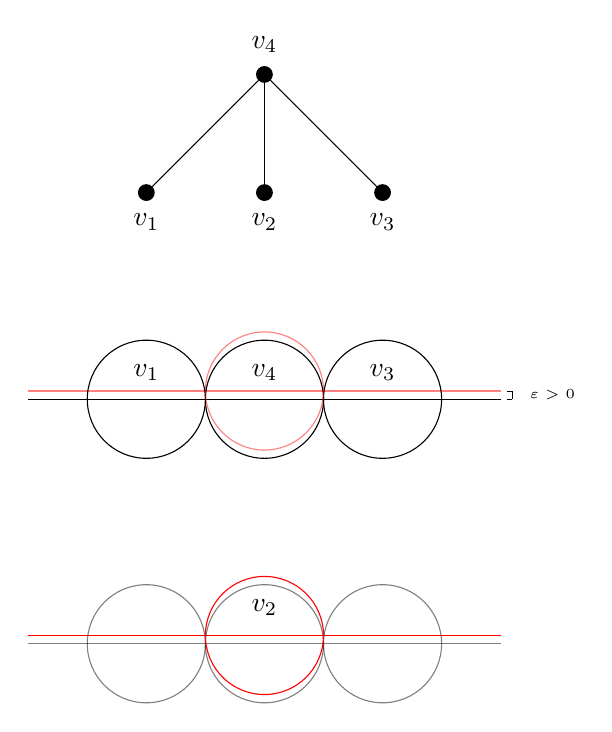
\begin{tikzpicture}[scale=1.5]

\draw (-2,0) -- (2,0);
\draw[red ,opacity = 0.5] (-2,0.07) -- (2,0.07);
\draw  (-1,0) circle [radius=0.5];
\draw[color=black] (-1,0.2265) node {$v_1$};
\draw  (0,0) circle [radius=0.5];
\draw[color=black] (0,0.2265) node {$v_4$};
\draw  (1,0) circle [radius=0.5];
\draw[color=black] (1,0.2265) node {$v_3$};

\draw[red, opacity = 0.5] (0,0.07) circle [radius=0.5];
\draw[color=black] (2.4386,0.0367) node {\tiny $\varepsilon > 0$};

% lines to describe distance (epsilon)
\draw[very thin] (2.1,0.07) -- (2.1,0);
\draw[very thin] (2.05,0.07) -- (2.1,0.07);
\draw[very thin] (2.05,0) -- (2.1,0);

\draw[opacity = 0.5] (-2,-2.07) -- (2,-2.07);
\draw[red] (-2,-2) -- (2,-2);
\draw[opacity = 0.5]  (0,-2.07) circle [radius=0.5];
\draw[opacity = 0.5]  (1,-2.07) circle [radius=0.5];
\draw[opacity = 0.5]  (-1,-2.07) circle [radius=0.5];
\draw[red] (0,-2) circle [radius=0.5];
\draw[color=black] (0,-1.765) node {$v_2$};

\node[draw,circle,inner sep=2pt,fill,label distance=1cm] (v1) at (0,2.75) {};
\draw[color=black] (0,3) node {$v_4$};
\node[draw,circle,inner sep=2pt,fill,label distance=1cm] (v3) at (0,1.75) {};
\draw[color=black] (0,1.5) node {$v_2$};
\node[draw,circle,inner sep=2pt,fill,label distance=1cm] (v2) at (-1,1.75) {};
\draw[color=black] (1,1.5) node {$v_3$};
\node[draw,circle,inner sep=2pt,fill,label distance=1cm] (v4) at (1,1.75) {};
\draw[color=black] (-1,1.5) node {$v_1$};
\draw  (v1) edge (v2);
\draw  (v1) edge (v3);
\draw  (v1) edge (v4);
\end{tikzpicture}
\end{scaletikzpicturetowidth}
\caption{A construction of $K_{1,3}$ with a disk realization, being this graph a TSG.}
\label{fig:thinK13}
\end{figure}

\begin{theorem}[Hayashi et al. \cite{hayashiThinStripGraphs2017}]
  There is no constant $t$ such that SG($t$) = TSG.
\end{theorem}

\begin{theorem}[Hayashi et al. \cite{hayashiThinStripGraphs2017}]
  There is no constant $t$ such that SG($t$) = UDG.
\end{theorem}

Hayashi et al. left some open problems. I try to expand the knowledge around some of these problems
to better understand them, largely for the recognition of this class of graphs. Before that, we see where this class lays in the hierarchy of classes. We know by definition that TSG $\subsetneq$ UDG.

\subsection{Interval graphs}

Thin strip graphs shares their geometrical structure with interval graphs (remember SG($0$) = UIG). In this subsection, we overview the results of Hayashi et al. \cite{hayashiThinStripGraphs2017} where they find maximal and minimal superclasses for TSG in the interval graphs presented in chapter \ref{chap:interval}. The following theorem will be proven by taking the proof written by Hayashi et al. in order to use their mapping in other theorems (e.g. \ref{chap:twolevel}).

\begin{theorem}[Hayashi et al. \cite{hayashiThinStripGraphs2017}]
  \label{theo:muigTSG}
  MUIG $\subsetneq$ TSG.
\end{theorem}

\proof{
First, we prove that MUIG $\neq$ TSG. This can be proven because $C_4 \in$ TSG if we take as points $(0,0),(0,\varepsilon),(1,0),(1,\varepsilon)$ with $1 >\varepsilon > 0$ and $C_4 \notin$ MUIG because it is a chordal graph.

Then, we have to prove that MUIG $\subseteq$ TSG. Let $G = (V,E) \in$ MUIG where each vertex is a unit mixed interval denoted as $I_v$. We define $t = \min\{|I_u\cap I_v| : |I_u\cap I_v| > 0, \{I_u,I_v\} \subseteq V\}$ and $s = \min\{\ell(I_v) - r(I_u) : \ell(I_v) > r(I_u), \{I_u,I_v\} \subseteq V\}$. We have then $t$ being the minimum length of an intersection bigger than zero (that is, not endpoint-adjacent) and $s$ is the minimum distance between non-adjacent vertices (also not endpoint-adjacent). We also define $c(I_v) = \frac{\ell(I_v) + r(I_v)}{2}$ as the center of the interval and $p(I_v) = (-1)^{\left \lfloor{c(I_v)}\right \rfloor }$.

Let $d$ be a real such that $0 < d < \frac{2}{3}$, $d\leq \frac{t}{4}$, $d < \frac{s}{2}$ and $\varepsilon \geq 2\sqrt{d-d^2}$. If we let $h = \sqrt{d-d^2}$, then we can create a $2h$-realization of $G$ with the following mapping:

\[ \phi(v) =
  \begin{cases}
      (c(I_v),0) & \text{if}\  I_v\  \text{is a closed interval} \\
      (c(I_v),hp(I_v)) & \text{if}\  I_v\  \text{is an open interval} \\
      (c(I_v)-d,hp(I_v)) & \text{if}\  I_v\  \text{is a closed-open interval} \\
      (c(I_v)+d,hp(I_v)) & \text{if}\  I_v\  \text{is an open-closed interval}
   \end{cases}
\]

For two vertices $u$ and $v$ of $G$ such that $u \leq v$, we have the three following cases:

\begin{enumerate}
  \item $r(I_u) < \ell(I_v)$:

    $I_u$ and $I_v$ are not adjacents, which means that $\text{dist}(\phi(u),\phi(v)) > 1$.
    If we minimize the distance between them we have $\phi(u) = (c(I_u)+d,hp(I_u))$ and $\phi(v) = (c(I_v)-d,hp(I_v))$ with $p(I_u) = p(I_v)$. Therefore, we only have to compare their $x$-coordinates:

    $$\text{dist}(\phi(u),\phi(v)) \geq (c(I_v)-d) - (c(I_u)+d) = c(I_v)-c(I_u) - 2d$$

    By definition, $s \leq l(I_v)-r(I_u)$. If we take the centers, then $s \leq c(I_v)-c(I_u) -1$, which means finally that $s +1 \leq c(I_v)-c(I_u)$

    $$\text{dist}(\phi(u),\phi(v)) \geq s + 1 - 2d > 1$$

  \item $r(I_u) > \ell(I_v)$:
    In this case $u$ and $v$ are adjacent. We maximize $\text{dist}(\phi(u),\phi(v))$ when $\phi(u) = (c(I_u)-d,hp(I_u))$ and $\phi(v) = (c(I_v)+d,hp(I_v))$ with $p(I_u) \neq p(I_v)$. Therefore,

\[    \begin{split}
    \text{dist}(\phi(u),\phi(v)) & \leq \sqrt{((c(I_v)+d)-(c(I_u)-d))^2 + (h+h)^2} \\
     & \text{with the same reasoning as before}\  c(I_v)-c(I_u) \leq 1-t\\
     & \leq \sqrt{(1-t+2d)^2 + 4h^2} \\
     & \leq \sqrt{(1-4d+2d)^2 + 4(d-d^2)} \\
     & = \sqrt{1-4d+4d^2 + 4d-4d^2} = 1
    \end{split}
\]

  \item $r(I_u) = \ell(I_v)$:

  In this case, $u$ and $v$ are adjacent only if $r(I_u)$ and $I_v$ are closed. We know that $c(I_v) = c(I_u)+1$ and $p(I_u) \neq p(I_v)$. Without loss of generality, we suppose that $p(I_u) = 1$ and $p(I_v) = -1$. We have two cases:
  \begin{enumerate}
    \item Both ends are closed. So we have this set of possible assignments for each one of the vertices:

    $$\phi(u) \in \{(c(I_u),0), (c(I_u)+d,h)\}$$
    $$\phi(v) \in \{(c(I_u)+1,0), (c(I_u)+1-d,-h)\}$$
    This gives us a rectangle with its diagonal smaller than one.

\item One of the ends is closed, we suppose $r(I_u)$ is open. In this case, we have these solutions:

  $$\phi(u) \in \{(c(I_u)-d,h), (c(I_u),h)\}$$
  $$\phi(v) \in \{(c(I_u)+1,0), (c(I_u)+1,-h), (c(I_u)+1\pm d,-h)\}$$

  Every distance between every points is greater than 1 if we take into consideration the domain of $d$. \qed

  \end{enumerate}
\end{enumerate}
}

Thin strip graphs can also be seen as unfettered unit interval graphs, which means that if a graph is a thin strip graph, then we can partition this graph with a level structure where each level is a clique. This information will be relevant in the next section.

\begin{theorem}[Hayashi et al. \cite{hayashiThinStripGraphs2017}]
  TSG $\subsetneq$ UUIG.
\end{theorem}

\proof{See \cite{hayashiThinStripGraphs2017}.}


\section{Characterization of thin strip graphs}

One of the main goals of this thesis is to characterize thin strip graphs by forbidden induced subgraphs. We know that TSG is an hereditary class, then a way to characterize this class of graphs is by looking for its forbidden subgraphs the same way as MUIG has been characterized by Joos. Furthermore, MUIG $\subsetneq$ TSG by Theorem \ref{theo:muigTSG}, so the first we can do is to check if the forbidden subgraphs of MUIG are also for TSG.

One of the main goals of this thesis is to characterize TSG. by forbidden induced subgraphs. To approach this, we will see how many induced forbidden subgraphs are also forbidden for TSG. We have described the familes of forbidden induced subgraphs for MUIG in section \ref{sec:muig} and one of these familes has been proven to be a forbidden induced subgraph for TSG.

\subsection{Mixed unit interval graph forbidden subgraphs}

\begin{theorem}[Hayashi et al. \cite{hayashiThinStripGraphs2017}]
  $\mathcal{R}$ is a forbidden induced subgraph family of TSG.
\end{theorem}

\begin{proof}
  We can prove that $\mathcal{R} \notin$ UUIG because TSG $\subsetneq$ UUIG. We can prove this by taking into consideration the display of the graphs in Figure \ref{graphsR}.

  Let $v$ be the leftmost vertex of $R_k$ with $k \in \mathbb{N}$. We have two choices:

  \begin{itemize}
    \item $v\in L_1 = K_1$: we have $H = R_k\setminus L_1$.
    $H$ has only one connected component, which means that it is a valid level. The next step is to take $N(L_1 \cap H) = L_2$, then $N(L_2 \cap H') = L_3$ where $H' = H\setminus L_2$.We repeat this until we arrive to the end of our graph. The last one will divide the graph in two components of $K_1$, which does not respect our condition because $L_n$ has already one adjacent level ($L_{n-1}$).
    \item $v\in L_1' = K_2$: in this case $H$ has two connected components, $K_1$ and $H\setminus K_1$. This level is valid, however, because it has two components $L_1'$ cannot be the first level of our level structure, so we take the neighbour $K_1$ as the first level $L_1$. We can observe that we are in the same spot as in the previous case, where $L_1 = K_1$.
  \end{itemize}

  Another (more extended) proof can be found in \cite{hayashiThinStripGraphs2017}.
\end{proof}

We see that $\mathcal{R}$ is a class of forbidden subgraphs of TSG. Nevertheless, the rest of the forbidden subgraphs for MUIG are thin strip graphs. The main reason is because they are unfettered unit interval graphs. We see our first example with the forbidden graph for MUIG $F$.

\begin{figure}
\begin{center}
  \begin{scaletikzpicturetowidth}{\textwidth}
  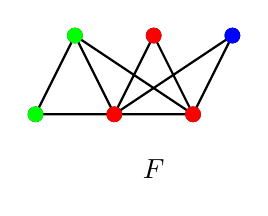
\begin{tikzpicture}[scale=1]
    \def\ver{0.1} %size of a vertex
    \def\x{1}

    \def\xa{0}
    \def\ya{0}

    %G_1
    \path[fill] (\xa+1,\ya) circle (\ver);
    \path[fill] (\xa+2,\ya) circle (\ver);
    \path[fill] (\xa+0.5,\ya+1) circle (\ver);
    \path[fill] (\xa+1.5,\ya+1) circle (\ver);
    \path[fill] (\xa+2.5,\ya+1) circle (\ver);
    \path[fill] (\xa,\ya) circle (\ver);

    \draw[thick] (\xa+1,\ya)--(\xa+2,\ya)
    (\xa+1,\ya)--(\xa+0.5,\ya+1)--(\xa+2,\ya)
    (\xa+1,\ya)--(\xa+2.5,\ya+1)--(\xa+2,\ya)
    (\xa+1,\ya)--(\xa+1.5,\ya+1)--(\xa+2,\ya)
    (\xa+1,\ya)--(\xa,\ya)--(\xa+0.5,\ya+1);

    \path[fill=red] (\xa+1,\ya) circle (\ver);
    \path[fill=red] (\xa+2,\ya) circle (\ver);
    \path[fill=green] (\xa+0.5,\ya+1) circle (\ver);
    \path[fill=red] (\xa+1.5,\ya+1) circle (\ver);
    \path[fill=blue] (\xa+2.5,\ya+1) circle (\ver);
    \path[fill=green] (\xa,\ya) circle (\ver);

    \node (1) at (\xa+1.5,\ya-0.7) {$F$};

\end{tikzpicture}
\end{scaletikzpicturetowidth}
\end{center}
\caption{The graph $F$ where each level is represented by a different color.}\label{fig:graphF_clique}
\end{figure}

\begin{theorem}
  $F \in$ TSG.
\end{theorem}

\proof{
To prove this we have to find an $\epsilon$-realization for our graph $F = (V,E)$ with $\varepsilon$ arbitrarily small. Let $\phi(v)$ be the mapping of our vertices on the plane. We know that the level structure of $F$ is $L = \{L_1 = K_2, L_2=K_3, L_3=K_1\}$ as seen in Figure \ref{fig:graphF_clique}. For each $v_k \in L_2$ with $k\in [0,2]$ as follows:

$$\phi(v_k) = \Bigg(0, \varepsilon \frac{k}{2}\Bigg)$$

Then, for each $u_k \in L_1$ with $l\in [1,2]$ as follows if we take into consideration that $v_0u_0, v_1u_0, v_0u_1 \in E$:

$$\phi(u_1) = \Bigg(\Big(\frac{\varepsilon}{4}\Big)^2 -1, \varepsilon \frac{1}{4}\Bigg)$$
$$\phi(u_2) = (-1, 0)$$


If you can see $L_1$ at the left of $L_2$. Finally, we have $w\in L_3$. We can see that $w$ and $u_1$ share the same neighbours, so they can be put in the same
$y$-coordinate we put it at the right side of $L_3$.

$$\phi(w) = \Bigg(1 - \Big(\frac{\varepsilon}{4}\Big)^2, \varepsilon \frac{1}{4}\Bigg)$$ \qed
}

We prove the same thing for $\mathcal{T}$ with the same procedure:


\begin{figure}[t]
\begin{center}
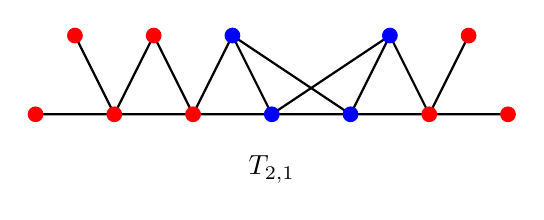
\begin{tikzpicture}[scale=1]
\def\ver{0.1} %size of a vertex
\def\x{1}

\def\xa{0}
\def\ya{0}

\def\xb{4}
\def\yb{0}

\def\xc{9}
\def\yc{0}

\def\xd{3}
\def\yd{-2.5}

\draw[thick] (\xc,\yc)--(\xc+6,\yc)
(\xc+0.5,\yc+1)--(\xc+1,\yc)--(\xc+1.5,\yc+1)--(\xc+2,\yc)--(\xc+2.5,\yc+1)--(\xc+3,\yc)--(\xc+4.5,\yc+1)
(\xc+5.5,\yc+1)--(\xc+5,\yc)--(\xc+4.5,\yc+1)--(\xc+4,\yc)--(\xc+2.5,\yc+1);

%graph T_{2,1}
\path[fill=red] (\xc,\yc) circle (\ver);
\path[fill=red] (\xc+1,\yc) circle (\ver);
\path[fill=red] (\xc+2,\yc) circle (\ver);
\path[fill=blue] (\xc+3,\yc) circle (\ver);
\path[fill=blue] (\xc+4,\yc) circle (\ver);
\path[fill=red] (\xc+5,\yc) circle (\ver);
\path[fill=red] (\xc+6,\yc) circle (\ver);
\path[fill=red] (\xc+0.5,\yc+1) circle (\ver);
\path[fill=red] (\xc+1.5,\yc+1) circle (\ver);
\path[fill=blue] (\xc+2.5,\yc+1) circle (\ver);
\path[fill=blue] (\xc+4.5,\yc+1) circle (\ver);
\path[fill=red] (\xc+5.5,\yc+1) circle (\ver);


\node (1) at (\xc+3,\yc-0.7) {$T_{2,1}$};


\end{tikzpicture}
\end{center}
\caption{The graph $T_{2,1}$ with the diamond in blue and the arms in red.}\label{fig:graph_T_clique}
\end{figure}

\begin{theorem}
  $\mathcal{T} \subset$ TSG.
\end{theorem}

\proof{begin proving}

\section{Recognition}

The recognition of this class of graphs is stated by Breu in his thesis \todo{explain everything about dangerous cycles and
complement oriented graphs in Breu's paper}.
